In this section we connect three load generating VMs to two middlewares and three memchached servers. We want to understand the effects of increasing the multi-get size on the performance of system. In addition, we analyze if sharding the multigets improves the performance.

\subsection{Sharded Case}
The overview of the experiment parameters is given in the following table:
\begin{center}
	\scriptsize{
		\begin{tabular}{|l|c|}
			\hline Number of servers                & 3                       \\ 
			\hline Number of client machines        & 3                       \\ 
			\hline Instances of memtier per machine & 2                       \\ 
			\hline Threads per memtier instance     & 1                       \\
			\hline Virtual clients per thread       & 2     		            \\ 
			\hline Workload                         & ratio=1:$<$Multi-Get size$>$             \\
			\hline Multi-Get behavior               & Sharded                 \\
			\hline Multi-Get size                   & \{1,3,6,9\}                 \\
			\hline Number of middlewares            & 2                       \\
			\hline Worker threads per middleware    & 64 \\
			\hline Repetitions                      & 3                \\ 
			\hline 
		\end{tabular}
	} 
\end{center}

% plots
If sharding is activated, the keys inside the multiget requests are evenly split by the workers and distributed among the servers.
The average response time measured on the client as a function of the multiget size and the percentiles for the sharded case are shown in Figures \ref{sharded_rt} and \ref{sharded_percentiles}.
% data: [2018-11-22_18h12]
\begin{figure}[H]
   \begin{minipage}{0.48\textwidth}
     \centering
     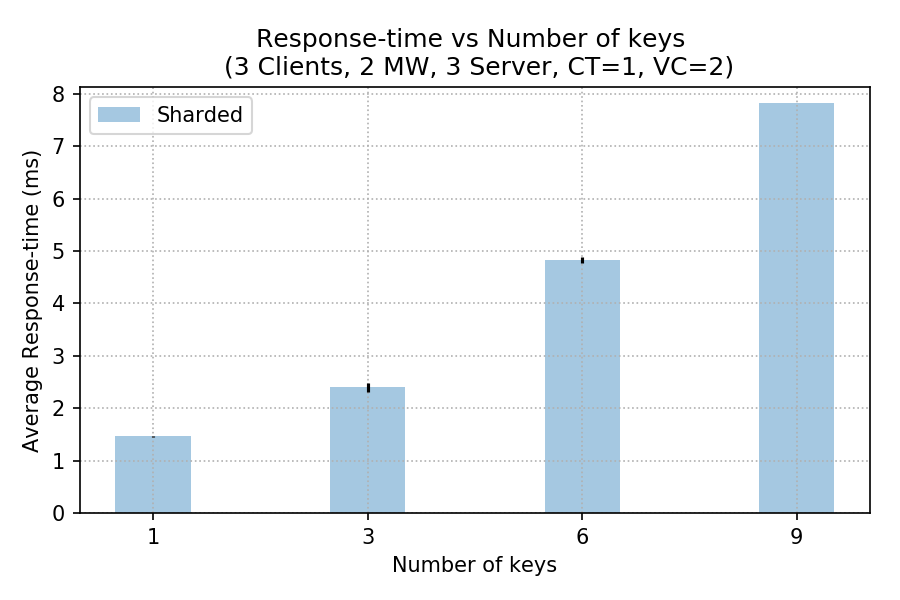
\includegraphics[width=1\linewidth]{figures/4_GetsAndMultigets/mem_rt_sharded_2018-11-22_18h12.png}
     \caption{Response time measured on clients.}\label{sharded_rt}
   \end{minipage}\hfill
   \begin{minipage}{0.48\textwidth}
     \centering
     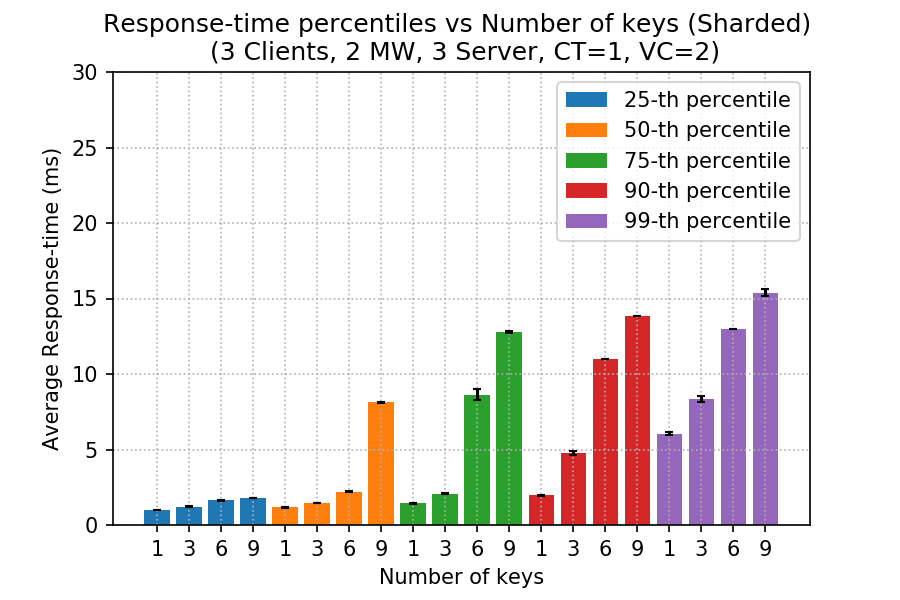
\includegraphics[width=1\linewidth]{figures/4_GetsAndMultigets/mem_perc_sharded_2018-11-22_18h12.png}
     \caption{Response time percentiles measured on client.}\label{sharded_percentiles}
   \end{minipage}
\end{figure}
First of all note that since we are in a closed system and we only have 12 clients, at least 52 workers will be idle at any moment in time. This is not optimal because threads use up memory and we establish more connections to servers than necessary (this depends on how the middleware has been implemented, but in our case the threads are started a priori). 

% bottleneck analysis
For 3, 6 and 9 keys the bottleneck is the outbound network bandwidth at the server VMs, as can be seen in Figure \ref{sharded_netsend_server}. Note that the maximal outbound network bandwidth of a server VM is 12 MBps.
For 1 key, the system is under-saturated because no component reaches full utilization. We checked the CPU usage of the VMs, the network send activity of the VMs, the response time breakdown in the middleware, the average queue length and we also have enough workers because at least 52 workers are always idle.\footnote{Those plots are not included in the report to keep it concise, but they can be found in the repository.} Thus for the 1 key case, the number of clients could be further increased to reach better performance regarding throughput.

\begin{figure}[H]
   \begin{minipage}{0.48\textwidth}
    \centering
	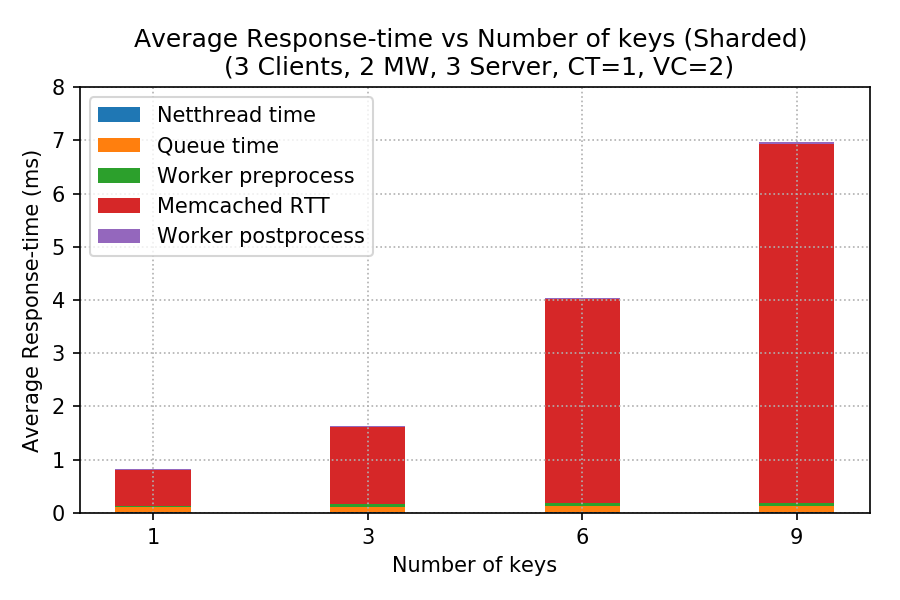
\includegraphics[scale=0.48]{figures/4_GetsAndMultigets/rt_breakdown_sharded_2018-11-22_18h12.png}
	\caption{Response time breakdown at middleware.}
	\label{rt_breakdown_sharded}
   \end{minipage}\hfill
   \begin{minipage}{0.48\textwidth}
     \centering
     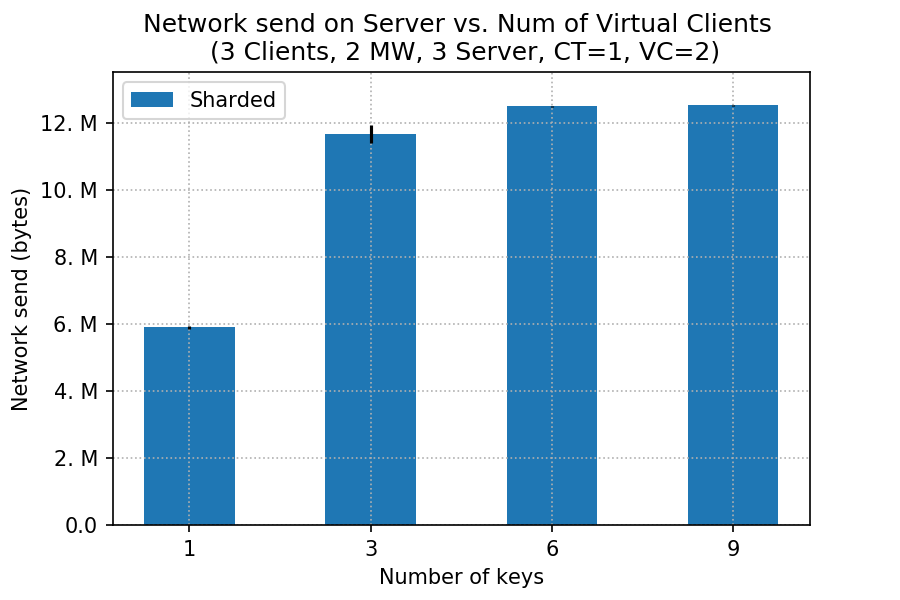
\includegraphics[width=1\linewidth]{figures/4_GetsAndMultigets/dstat_server_netsend_sharded_True_2018-11-22_18h12.png}
     \caption{Network send activity on a server VM.}\label{sharded_netsend_server}
   \end{minipage}
\end{figure}
If we look at the response time breakdown at the middleware in Figure \ref{rt_breakdown_sharded}, we can see that the memcached RTT makes up most of the time. The memcached RTT mainly consists of the network latency between the middleware and the server, the waiting time at the server because of the bandwidth bottleneck and the time it takes the server to write the response into the network. We see that the average response time on the middleware (Figure \ref{rt_breakdown_sharded}) is lower than on the client (Figure \ref{sharded_rt}), which is because of the network latency between the client and middleware. We also see that in Figures \ref{sharded_rt} and \ref{rt_breakdown_sharded}, the response time increases with the number of keys. This is because the server has to write more data into the network and also has to process more data. Note that the memcached RTT is what significantly increases the overall response time with increasing key size. 

If we look at the percentile plot (Figure \ref{sharded_percentiles}), we see that individual percentiles increase with increasing number of keys for the same reason as the average response time increases with the number of keys. 
The percentile plot will be further explained in comparison with the plot of the non-sharded case and in subsection \ref{sub:hist}.

\subsection{Non-sharded Case}
The overview of the experiment parameters is given in the following table:
\begin{center}
	\scriptsize{
		\begin{tabular}{|l|c|}
			\hline Number of servers                & 3                       \\ 
			\hline Number of client machines        & 3                       \\ 
			\hline Instances of memtier per machine & 2                       \\ 
			\hline Threads per memtier instance     & 1                       \\
			\hline Virtual clients per thread       & 2     		            \\ 
			\hline Workload                         & ratio=1:$<$Multi-Get size$>$             \\
			\hline Multi-Get behavior               & Non-Sharded                 \\
			\hline Multi-Get size                   & \{1,3,6,9\}                 \\
			\hline Number of middlewares            & 2                       \\
			\hline Worker threads per middleware    & 64 \\
			\hline Repetitions                      & 3                \\ 
			\hline 
		\end{tabular}
	} 
\end{center}

% plots
The average response time measured on the client as a function of the multiget size and the percentiles for the non-sharded case is shown in Figure \ref{nonsharded_rt} and \ref{nonsharded_percentiles}.
% data: [2018-11-22_18h12]
\begin{figure}[H]
   \begin{minipage}{0.48\textwidth}
     \centering
     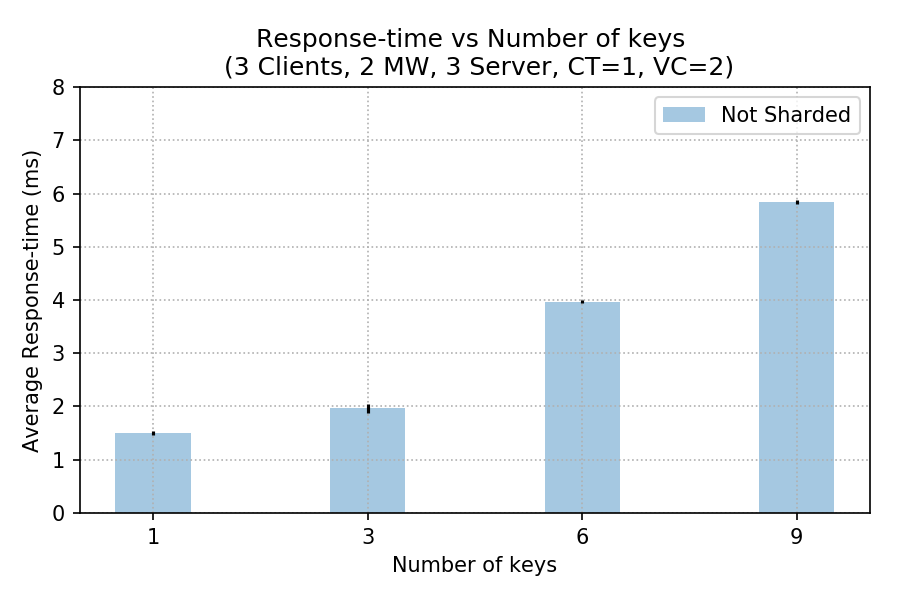
\includegraphics[width=1\linewidth]{figures/4_GetsAndMultigets/mem_rt_nonsharded_2018-11-22_18h12.png}
     \caption{Response time measured on clients.}\label{nonsharded_rt}
   \end{minipage}\hfill
   \begin{minipage}{0.48\textwidth}
     \centering
     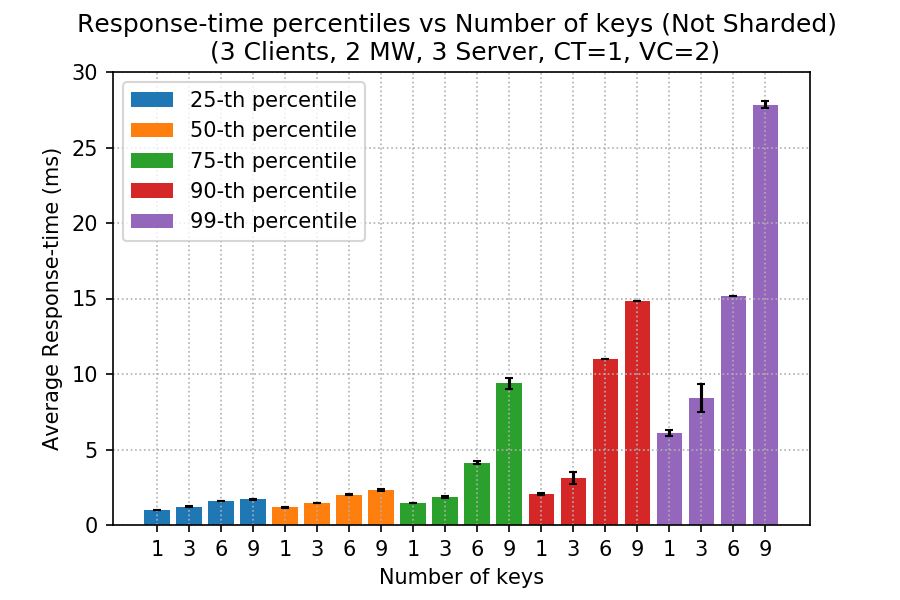
\includegraphics[width=1\linewidth]{figures/4_GetsAndMultigets/mem_perc_nonsharded_2018-11-22_18h12.png}
     \caption{Response time percentiles measured on client.}\label{nonsharded_percentiles}
   \end{minipage}
\end{figure}
For the non-sharded case we have the same bottleneck as in the sharded case, namely the outbound network bandwidth of the server VMs (see Figure \ref{nonsharded_netsend_server}). The same reasoning done in the sharded subsection applies here. For 1 key, the system is also under-saturated because no component reaches full utilization.  The memcached RTT makes up most of the response time measured at the middleware (Figure \ref{rt_breakdown_nonsharded}) and the response times increase with the key size for the same reasons. In this subsection I mainly focus on comparing the plots with their sharded counterpart. 


\begin{figure}[ht]
   \begin{minipage}{0.48\textwidth}
    \centering
	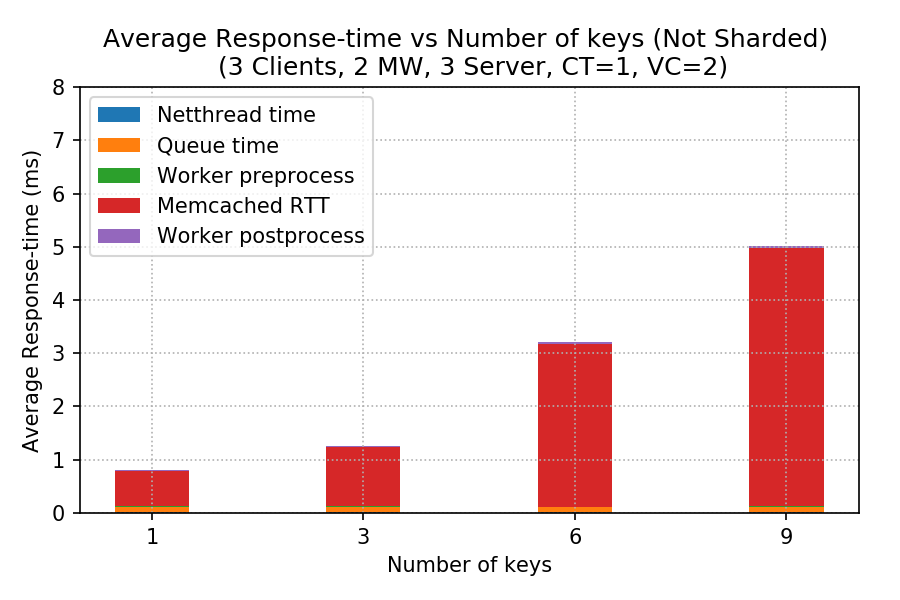
\includegraphics[scale=0.48]{figures/4_GetsAndMultigets/rt_breakdown_notsharded_2018-11-22_18h12.png}
	\caption{Response time breakdown at middleware.}
	\label{rt_breakdown_nonsharded}
   \end{minipage}\hfill
   \begin{minipage}{0.48\textwidth}
     \centering
     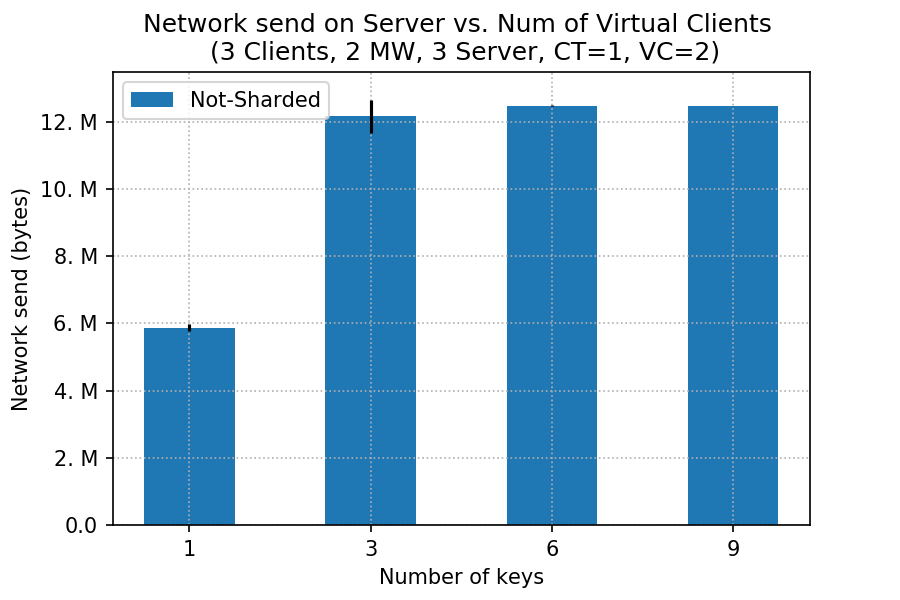
\includegraphics[width=1\linewidth]{figures/4_GetsAndMultigets/dstat_server_netsend_sharded_False_2018-11-22_18h12.png}
     \caption{Network send activity on a server VM.}\label{nonsharded_netsend_server}
   \end{minipage}
\end{figure}
First of all, looking at the requests with one key (Figures \ref{sharded_rt} and \ref{nonsharded_rt}), we see very similar response times for the sharded and non-sharded case because for one key the sharding behaves the same as for non-sharding.  For 3, 6 and 9 keys, we can observe that the average response times are higher in the sharded case than in the non-sharded case (Figures \ref{sharded_rt} and \ref{nonsharded_rt}). This is because in the sharded case a worker has to wait for a response from all servers, i.e. the response time is bound by the slowest server or rather the longest network latency to a server. In this experiment, the network latency between the middlewares and servers does not vary a lot (verified with ping logs), but I guess that if for example the latency to one server was a lot bigger then the other latencies, the effect would be even more significant. 

Even though in Figures \ref{rt_breakdown_sharded} and \ref{rt_breakdown_nonsharded} we can barely see any latencies other than the memcached RTT, looking at the numbers we observe that the worker preprocessing time is 5x bigger in the sharded case than in the non-sharded case. This is because a multiget request is divided into multiple requests and has to be copied into buffers before sending it to the servers while for the non-sharded case we can just take the buffer and send it to the server. But this time is negligible compared to the memcached RTT. 

%percentiles
Looking at the percentiles plots (Figures \ref{sharded_percentiles} and \ref{nonsharded_percentiles}), we have a larger deviation between percentiles in the non-sharded case than in the sharded case. This is because the response time in the non-sharded case depends on the server, which is chosen based on round-robin, while in the sharded case we are always limited by the slowest server, which leads to less variation in response time.

\subsection{Histogram} \label{sub:hist}
In this subsection we  look at the case with 6 keys inside the multigets, and present four histograms representing the sharded and non-sharded response time distribution, both as measured on the client, and inside the middleware. The bucket size is chosen to be 0.1ms. The histograms can be seen in Figure \ref{histograms}.
% plots: add all 4 in one place s.t can compare
\begin{figure}[ht]
        \centering
        \begin{subfigure}[b]{0.475\textwidth}
            \centering
            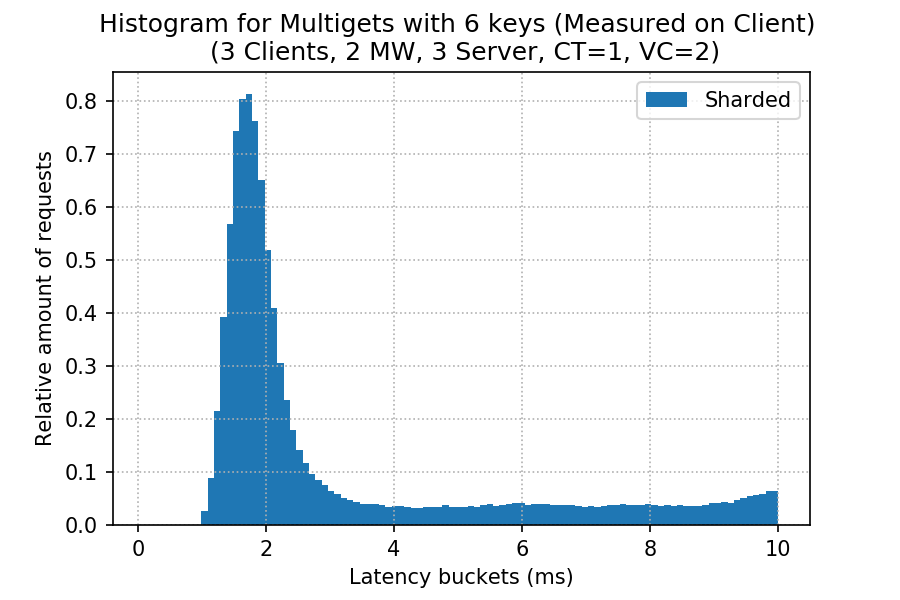
\includegraphics[width=\textwidth]{figures/4_GetsAndMultigets/mem_histogram_sharded_2018-11-22_18h12.png}
        \end{subfigure}
        \hfill
        \begin{subfigure}[b]{0.475\textwidth}  
            \centering 
            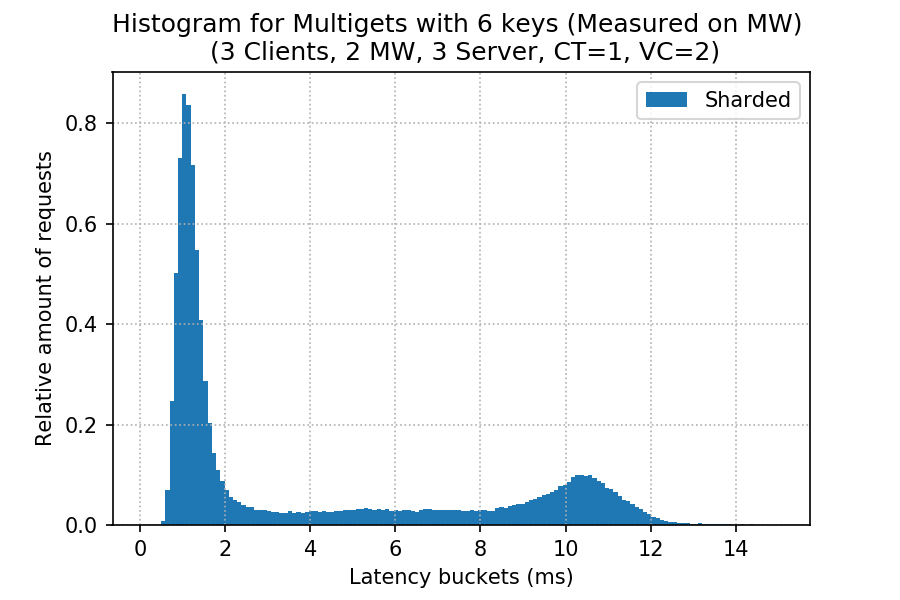
\includegraphics[width=\textwidth]{figures/4_GetsAndMultigets/mw_histogram_sharded_2018-11-22_18h12.png}
        \end{subfigure}
        \vskip\baselineskip
        \begin{subfigure}[b]{0.475\textwidth}   
            \centering 
            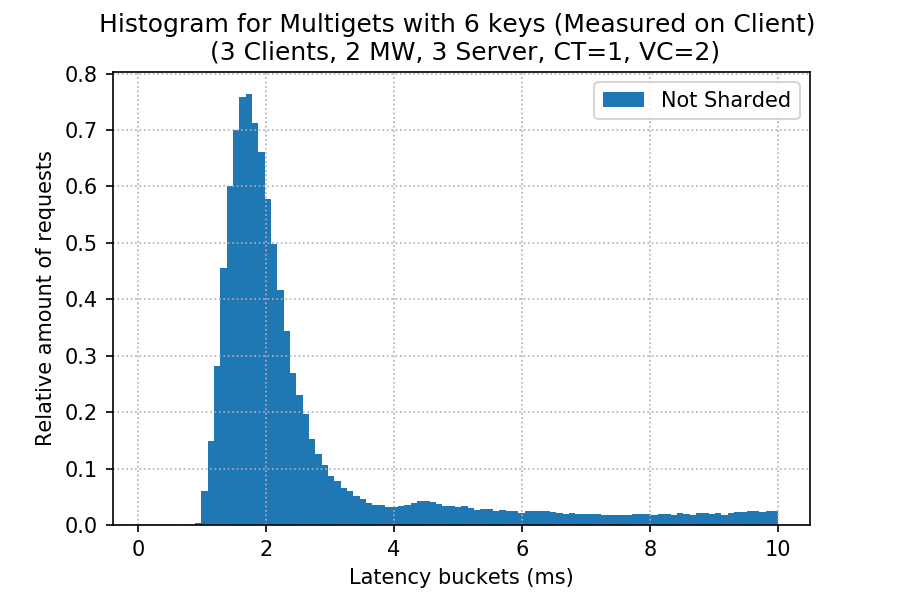
\includegraphics[width=\textwidth]{figures/4_GetsAndMultigets/mem_histogram_nonsharded_2018-11-22_18h12.png}
        \end{subfigure}
        \quad
        \begin{subfigure}[b]{0.475\textwidth}   
            \centering 
            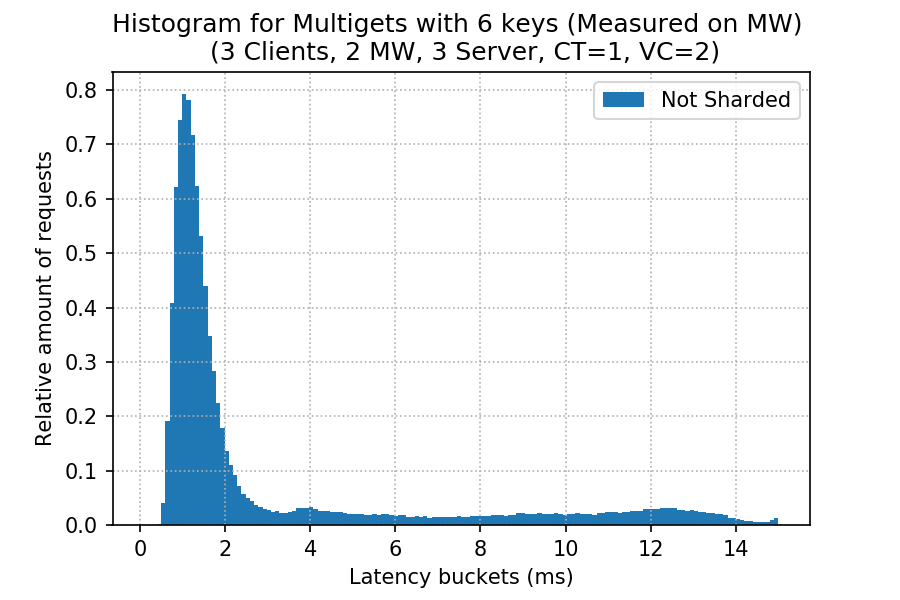
\includegraphics[width=\textwidth]{figures/4_GetsAndMultigets/mw_histogram_nonsharded_2018-11-22_18h12.png}
        \end{subfigure}
         \caption[]
        {\small Histograms of the response time distribution of sharded and non-sharded multigets measured on the client (left column) and on the middleware (right column). } 
        \label{histograms}
    \end{figure}
    
% explain
Generally we can say that the majority of requests are processed within 3ms for both the sharded and the non-sharded case. Also the histogram plots conform with the percentile plots. For the sharded-case we have 50\% of request being processed within 2ms, 75\% within 9ms, 90\% within 11ms and 99\% within 13ms. For the non-sharded case we have 50\% of request being processed within 2ms, 75\% within 4ms, 90\% within 15ms and 99\% within 15ms. In the sharded case, the 75th and 90th percentiles are significantly larger than in the non-sharded case, which is because in the sharded case we have a hill around 11ms, which will be explained later.

Comparing the client plots with the middleware plots, we see that the peak of the middleware plots is closer to  0ms than on the client plot. This is because of the network latency between the clients and middlewares which is not included in the middleware response time. We can also see that the distributions on the middleware are a little more narrow than on the clients. This is because the response time measured on clients captures a longer route of requests than the response time measured on the middlewares and thus we have more variability in the response time. Note that we had to cut the distributions measured on clients at 10ms because memtier did increase the bucket size from 0.1ms to 1ms after 10ms, which is too coarse grained. But essentially the continuation of the distributions can be seen in the middleware plots.

Comparing the sharded plots with the non-sharded plots, we can see that in the non-sharded case the distribution around the peak is more spread out than in the sharded case. This is because in the non-sharded case the response time of a request depends on the chosen server by the round-robin load balancer, which is not the same for every request, whereas in the sharded case, the response time is always determined by the slowest server and thus the response time of all requests is bound by this server, which leads to a more narrow distribution around the peak. Since the network latency between a middleware and a server is around 1ms for all servers, we only have one peak in the non-sharded case but I would expect multiple peaks if we had larger differences in latencies. 

What remains to be mention is the small hill around 10ms in the sharded case. I assume this is because of the bottleneck at the server which leads to congestion and thus to some requests having to wait longer than others to get processed. The hill almost disappeared in the non-sharded case, which might be because the probability for this delay at the server is smaller due to a request only involving one server and not all servers. This would support the hypothesis. 

\subsection{Summary}
%Compare the two modes with each other (for which multiget size is sharding preferred)
To conclude, non-sharding might be preferred over sharding because of a better average response time. This is because in the non-sharded case not all multigets are limited by the slowest server or largest latency to a server like in the sharded case. Also, sharding has an overhead of dividing multigets, combining responses and sending respectively receiving data from three instead of one server. The larger the service time differences between the servers and the network latency differences to the servers are, the bigger the average response time difference between the sharded and non-sharded case would be for the number of keys analyzed in this section.